\documentclass[a4paper,12pt]{article}
\setlength{\headheight}{68.803pt}
\addtolength{\topmargin}{-56.803pt}

\usepackage[utf8]{inputenc}
\usepackage[T1]{fontenc}
\usepackage{lmodern}
\usepackage[nopatch=footnote]{microtype}
\usepackage{fvextra}
\DefineVerbatimEnvironment{Verbatim}{Verbatim}{
  breaklines=true,
  breakanywhere=true,
  frame=single,
  fontsize=\small
}

% margin settings
\usepackage[
  left=1in,
  right=1in,
  top=3cm,
  bottom=1in
]{geometry}

\usepackage[
    colorlinks=true,
    linkcolor=black,
    urlcolor=blue,
    citecolor=blue,
    pdfborder={0 0 0},
    pdfauthor={Massimo Mantineo},
    pdftitle={Server TCP con I/O Multiplexing},
    pdfsubject={Laboratorio di Reti e Sistemi Distribuiti: HANDS-ON 3},
]{hyperref}

\usepackage{graphicx}
\graphicspath{{../../assets/}}
\usepackage{tikz}
\usetikzlibrary{positioning, arrows.meta}
\usepackage{listings}
\usepackage{xcolor}
\usepackage{amsmath, amssymb}
\usepackage{fancyhdr}
\usepackage{setspace}
\usepackage{pgfplots}
\pgfplotsset{compat=1.17}
\usepackage{booktabs}
\usepackage[skins, listings]{tcolorbox}
\usepackage{float}

\newtcblisting{terminal}[1][]{
    listing only,
    colback=black!85!white,
    colframe=black!70!white,
    colupper=green!80!white,
    coltitle=white,
    title=#1,
    fonttitle=\bfseries\sffamily,
    listing options={
        language={},
        basicstyle=\ttfamily\small\color{green!80!white},
        backgroundcolor={},
        frame=none,
        breaklines=true,
        showstringspaces=false,
        numbers=none
    },
    enhanced,
    drop shadow,
    arc=3mm
}

\newtcblisting{ccode}[1][]{
    listing only,
    colback=blue!3!white,
    colframe=blue!70!black,
    title=#1,
    fonttitle=\bfseries\sffamily,
    listing options={
        style=cstyle,
        backgroundcolor={},
        frame=none
    },
    enhanced,
    drop shadow,
    arc=3mm
}

\setlength{\footskip}{50pt}

% settings for C listings
\lstdefinestyle{cstyle}{
    language=C,
    basicstyle=\ttfamily\small,
    numbers=left,
    numberstyle=\tiny,
    stepnumber=1,
    numbersep=5pt,
    backgroundcolor=\color{white},
    showspaces=false,
    showstringspaces=false,
    showtabs=false,
    frame=single,
    tabsize=4,
    captionpos=b,
    breaklines=true,
    breakatwhitespace=true,
    keywordstyle=\color{blue}\bfseries,
    commentstyle=\color{green!50!black},
    stringstyle=\color{red},
}
\lstset{style=cstyle}

% Header and Footer
\pagestyle{fancy}
\fancyhf{}

\fancyhead[L]{%
  \parbox[b]{0.45\textwidth}{%
    \small
    Student Name: Massimo Mantineo\\
    Student ID: 541924
    \vspace{20pt}
  }%
}
\fancyhead[C]{%
  \parbox[b]{0.2\textwidth}{%
    \centering
    \normalsize \bfseries
    LabReSiD25\\
    Hands-On 3
    \vspace{20pt}
  }%
}
\fancyhead[R]{%
  \parbox[b]{0.35\textwidth}{%
    \flushright
    \includegraphics[width=3.5cm]{\detokenize{logo_unime_orizontale.png}}
    \vspace{15pt}
  }%
}

\renewcommand{\contentsname}{Indice}

\title{\vspace{-2cm}Relazione: Server TCP con I/O Multiplexing\\
\large (Hands-On 3)}
\author{Massimo Mantineo \\ Matricola: 541924}
\date{MESSINA, A.A. 2024/2025}

\begin{document}

% Cover page
\begin{titlepage}
    \thispagestyle{empty}
    \centering
    \vspace*{1cm}
    \includegraphics[width=6cm]{\detokenize{logo_unime_orizontale.png}}\par\vspace{1cm}
    \vspace{2cm}
    {\Large \textbf{Università degli Studi di Messina}\par}
    {\large Dipartimento MIFT - Corso di Laurea Triennale in Informatica (L-31)\par}
    \vspace*{1cm}
    {\large Laboratorio di Reti e Sistemi Distribuiti\par}
    \vspace{1cm}
    {\Large \textbf{HANDS-ON 3:}\\
    Server TCP con I/O Multiplexing\par}
    \vspace{2cm}
    {\large Massimo Mantineo \par}
    {\large Matricola: 541924 \par}
    \vfill
    {\large Messina, A.A. 2024/2025 \par}
\end{titlepage}

\clearpage
\pagestyle{fancy}
\tableofcontents
\newpage

\section{Problem Statement}
L'obiettivo della terza esercitazione (Hands-On 3) è il superamento dei limiti dei server iterativi tramite l'implementazione di un'architettura a **I/O Multiplexing**. Il sistema deve essere capace di gestire simultaneamente fino a 10 connessioni client utilizzando un unico thread di esecuzione. La sfida consiste nel monitorare dinamicamente lo stato di molteplici file descriptor e rispondere a ciascun client con un payload specifico (\texttt{ACK_MULTIPLEX_OK}), garantendo l'assenza di interferenze tra le sessioni e ottimizzando l'uso del tempo di CPU.

\section{Stato dell'Arte}
Il multiplexing è la risposta alla necessità di scalabilità senza l'overhead computazionale dei thread o della creazione di processi pesanti (\texttt{fork}).
\begin{itemize}
    \item \textbf{Gestione degli Eventi}: Invece di bloccarsi su un singolo socket, il server delega al kernel il monitoraggio di un set di FD. La syscall \texttt{select()} analizza tre maschere di bit (lettura, scrittura, eccezione) e ritorna quando almeno un evento è occorso.
    \item \textbf{Limiti della \texttt{select()}}: Sebbene portabile, la \texttt{select()} presenta un limite strutturale definito dalla costante \texttt{FD_SETSIZE} (solitamente 1024). Inoltre, la necessità di scansionare l'intero set ogni volta che la funzione ritorna rende la complessità lineare $O(N)$, dove $N$ è l'ID del descrittore più alto.
\end{itemize}

\section{Metodologia ed Implementazione}
L'architettura proposta si basa su un array statico di socket (\texttt{client_socket[10]}) e l'uso delle macro POSIX per la manipolazione degli \texttt{fd_set}.

\subsection{Algoritmo di Multiplexing}
Il server esegue un loop continuo in cui ricostruisce la maschera di lettura prima di ogni invocazione della \texttt{select()}:
\begin{ccode}[Snippet Gestione Descrittori]
FD_ZERO(&readfds);
FD_SET(master_socket, &readfds);
for (i = 0; i < MAX_CLIENTS; i++) {
    sd = client_socket[i];
    if (sd > 0) FD_SET(sd, &readfds);
    if (sd > max_sd) max_sd = sd;
}
activity = select(max_sd + 1, &readfds, NULL, NULL, NULL);
\end{ccode}

\subsection{Dispatching dei Task}
Dopo che la \texttt{select()} ritorna, il server distingue due rami logici:
\begin{enumerate}
    \item \textbf{Nuova Connessione}: Se \texttt{FD_ISSET(master_socket)}, viene eseguita la \texttt{accept()} e il nuovo FD viene memorizzato nel primo slot libero dell'array.
    \item \textbf{I/O Applicativo}: Se \texttt{FD_ISSET(sd)}, viene eseguita la \texttt{read()}. Se la lunghezza è 0, il client ha chiuso la socket; altrimenti, il messaggio viene processato.
\end{enumerate}

\section{Risultati}
La validazione è stata effettuata tramite uno script bash che lancia 5 client in background, verificando la corretta ricezione degli ACK sincronizzati.

\begin{figure}[H]
    \centering
    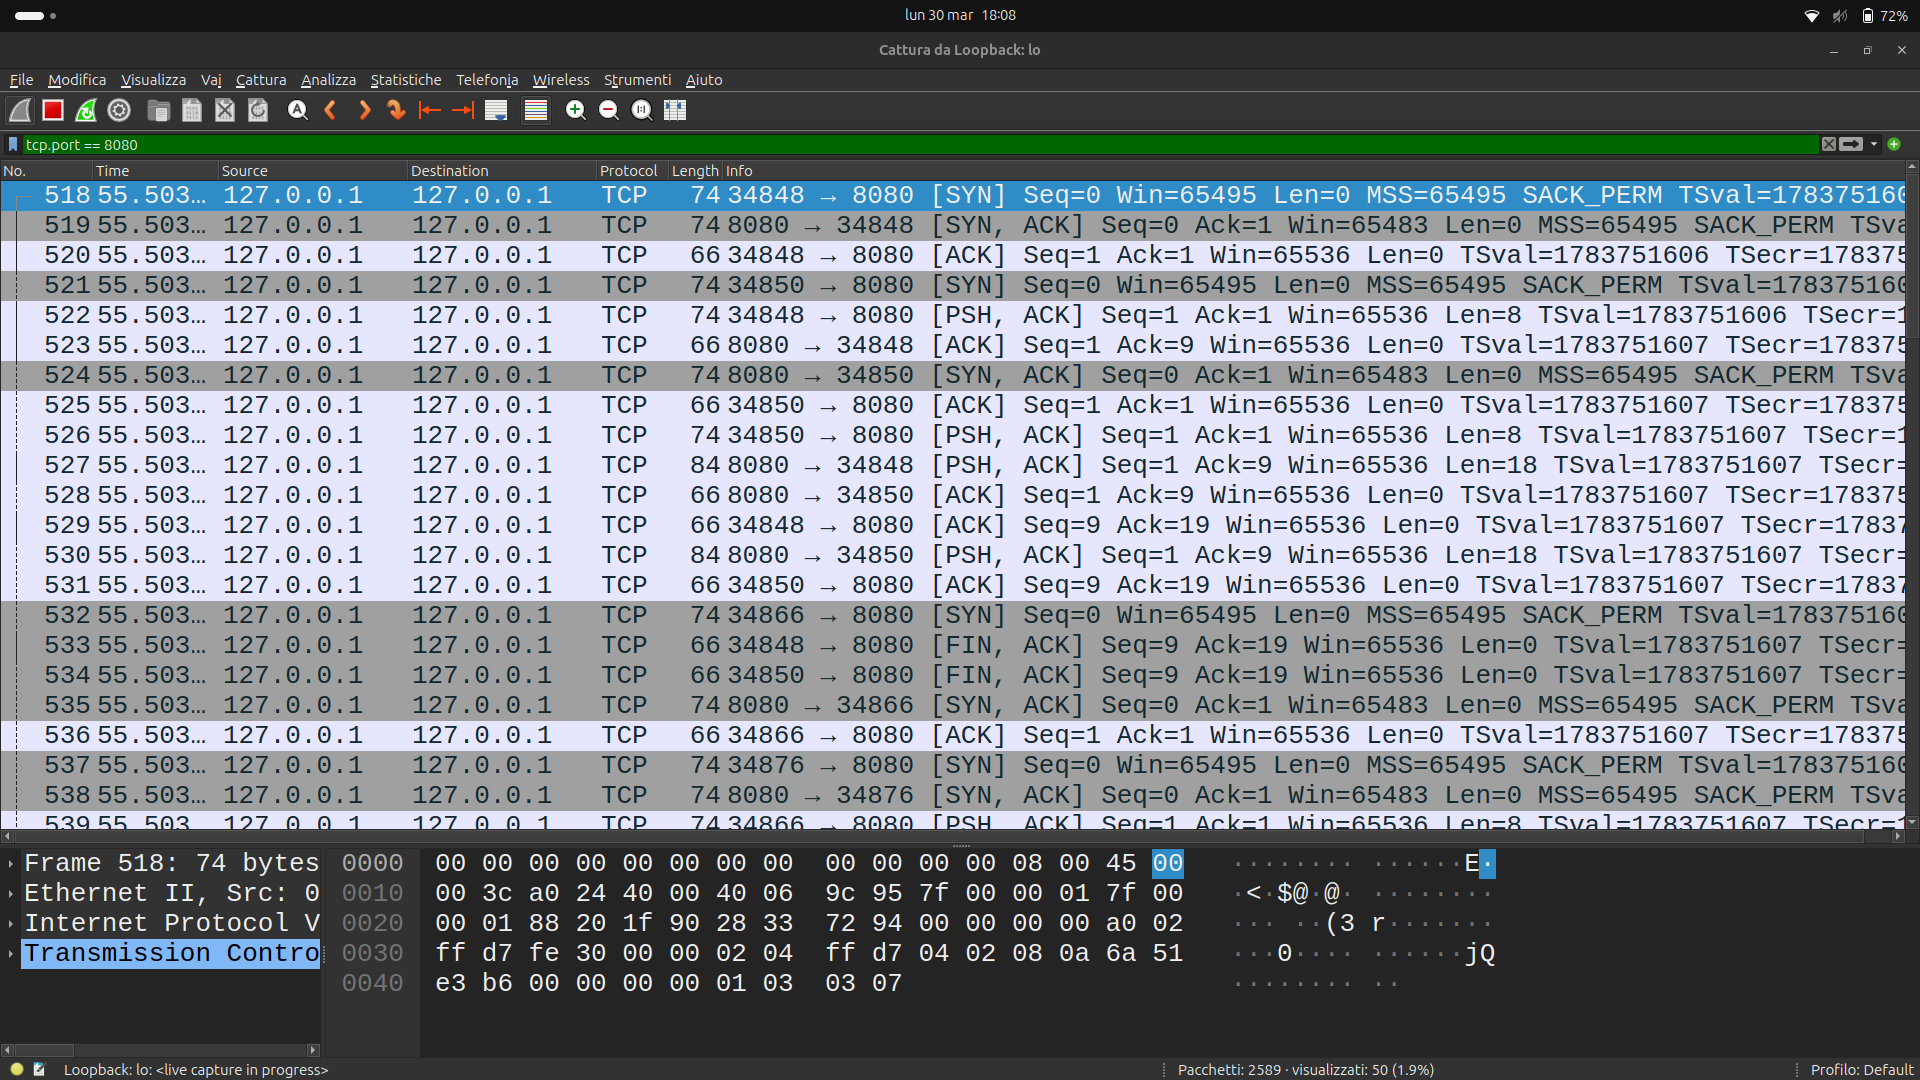
\includegraphics[width=0.9\textwidth]{ho3/ho3_wireshark_multiplexing.png}
    \caption{Gestione asincrona del Multiplexing su Wireshark.}
    \label{fig:ho3_multiplexing}
\end{figure}

\subsection{Analisi Wireshark}
L'ispezione dei pacchetti (Figura~\ref{fig:ho3_multiplexing}) mostra come il server gestisca gli handshake e gli scambi dati in modo asincrono. Nonostante le richieste arrivino in un lasso di tempo di millisecondi, il server risponde a ciascun client (porte sorgente 34848, 34850, ecc.) senza che l'elaborazione di uno blocchi l'altro.

\subsection{Osservazione sui Descrittori}
L'analisi dei log evidenzia come i file descriptor vengano riutilizzati efficientemente dal kernel una volta chiusi, mantenendo basso l'indice dell'array monitorato dalla \texttt{select()}.

\section{Conclusioni e Sviluppi Futuri}
L'Hands-On 3 ha confermato che il multiplexing è una soluzione robusta per server con numero di client moderato. L'approccio a singolo thread semplifica la gestione della memoria condivisa, eliminando la necessità di primitive di sincronizzazione (mutex).

\noindent \textbf{Sviluppi futuri:}
\begin{itemize}
    \item \textbf{Scalabilità}: Migrazione verso \texttt{epoll()} (Edge-Triggered) per superare i limiti di \texttt{FD_SETSIZE} in scenari di alto traffico.
    \item \textbf{Persistenza}: Implementazione di un protocollo applicativo con gestione del mantenimento dello stato (session tracking) tra invii consecutivi dello stesso client.
\end{itemize}

\end{document}
